\lab{Numerical Methods for Initial Value Problems}{Numerical Methods for Initial Value Problems}
\label{lab:ivp}
\labdependencies{IVPBVPIntro}

\objective{Implement several basic numerical methods for initial value problems (IVPs) and use them to study harmonic oscillators.}

\section*{Methods for Initial Value Problems}
Consider the \textit{initial value problem} (IVP)
\begin{align}
	\begin{split}
\x'(t) &= f(\x(t),t),\quad t_0 \leq t \leq t_f \\
\x(t_0) &= \x_0, 
	\end{split}
	\label{ivp:generic}
\end{align}
where $f$ is a suitably continuous function.
A solution of \eqref{ivp:generic} is a continuously differentiable, and possibly vector-valued, function $\x(t) = \left[x_1(t),\hdots,x_m(t)\right]\trp$, whose derivative $\x'(t)$ equals $f(\x(t),t)$ for all $t \in [t_0,t_f]$, and for which the \textit{initial value} $\x(t_0)$ equals $\x_0$.

Under the right conditions, namely that $f$ is uniformly Lipschitz continuous in $\x(t)$ near $\x_0$ and continuous in $t$ near $t_0$, \eqref{ivp:generic} is well-known to have a unique solution.
%[reference Volume 4 here].
However, for many IVPs, it is difficult, if not impossible, to find a closed-form, analytic expression for $\x(t)$.
In these cases, numerical methods can be used to instead \textit{approximate} $\x(t)$.

As an example, consider the initial value problem
\begin{align}
	\begin{split}
x'(t) &= \sin(x(t)), \\
x(0) &= x_0.
	\end{split}\label{ivp:example}
\end{align}
The solution $x(t)$ is defined implicitly by
\[t = \ln \left|\frac{\cos(x_0) + \cot(x_0)}{\csc(x(t)) + \cot(x(t))} \right|.\]
This equation cannot be solved for $x(t)$, so it is difficult to understand what solutions to \eqref{ivp:example} look like.
Since $sin(n\pi)=0$, there are constant solutions $x_n(t) = n \pi,$ $n \in \mathbb{Z}$.
Using a numerical IVP solver, solutions for different values of $x_0$ can be approximated.
Figure \ref{ivp:int_curves} shows several of these approximate solutions, along with some of the constant, or \textit{equilibrium}, solutions.

\begin{figure}[H]
\centering
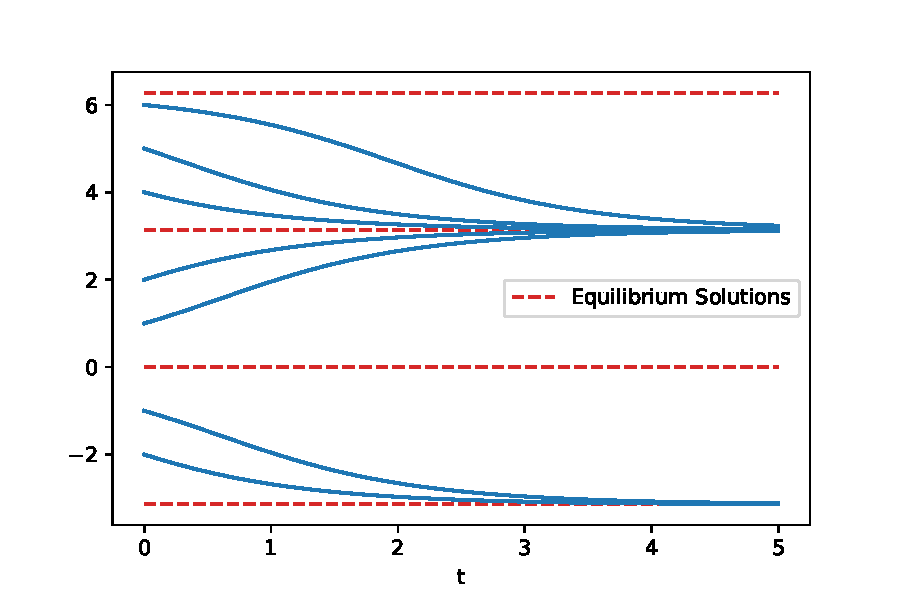
\includegraphics[width=\textwidth]{figures/example2.pdf}
\caption{Several solutions of \eqref{ivp:example}, using \li{scipy.integrate.odeint}. }
\label{ivp:int_curves}
\end{figure}


\section*{Numerical Methods}
For the numerical methods that follow, the key idea is to seek an approximation for the values of $\x(t)$ only on a finite set of values $t_0 < t_1 < \hdots < t_{n-1} < t_n \ (= t_f)$.
In other words, these methods try to solve for $\x_1,\x_2,\hdots,\x_n$ such that $\x_i \approx \x(t_i)$.

\subsection*{Euler's Method}
For simplicity, assume that each of the $n$ subintervals $[t_{i-1},t_i]$ has equal length $h = (t_f-t_0)/n$. $h$ is called the \textit{step size}.
Assuming $\x(t)$ is twice-differentiable, for each component function $x_j(t)$ of $\x(t)$ and for each $i$, Taylor's Theorem says that
\begin{align*}
x_j(t_{i+1}) &= x_j(t_{i}) + h x'_j(t_i) + \frac{h^2}{2} x''_j(c)\text{ for some } c \in [t_i,t_{i+1}].
\end{align*}
The quantity $\frac{h^2}{2} x''_j(c)$ is negligible when $h$ is sufficiently small, and thus $x_j(t_{i+1}) \approx x_j(t_i) + h x'_j(t_i)$.
Therefore, bringing the component functions of $\x(t)$ back together gives
\begin{align*}
\x(t_{i+1}) &\approx \x(t_i) + h \x'(t_i)  ,\\
&\approx \x(t_{i}) + h f(\x(t_i),t_i).
\end{align*}
This approximation leads to the \textit{Euler method}: Starting with $\x_0 = \x(t_0)$, $\x_{i+1} = \x_i +hf(\x_i,t_i)$ for $i = 0, 1, \hdots, n-1$.
Euler's method can be understood as starting with the point at $\x_0$, then calculating the derivative of $\x(t)$ at $t_0$ using $f(\x_0,t_0)$, followed by taking a step in the direction of the derivative scaled by $h$. Set that new point as $\x_1$ and continue.

It is important to consider how the choice of step size $h$ affects the accuracy of the approximation. Note that at each step of the algorithm, the \textit{local truncation error}, which comes from neglecting the $x''_j(c)$ term in the Taylor expansion, is proportional to $h^2$.
The error $||\x(t_i)-\x_i||$ at the \textit{ith} step comes from $i = \frac{t_i-t_0}{h}$ steps, which is proportional to $h^{-1}$, each contributing $h^2$ error.
Thus the \textit{global truncation error} is proportional to $h$.
Therefore, the Euler method is called a \textit{first-order method}, or a $\mathcal{O}(h)$ method.
This means that as $h$ gets small, the approximation of $\x(t)$ improves in two ways.
First, $\x(t)$ is approximated at more values of $t$ (more information about the solution), and second, the accuracy of the approximation at any $t_i$ is improved proportional to $h$ (better information about the solution).
\begin{comment}
Euler's method is a first order method, with error $\mathcal{O}(h^1)$.
% \begin{enumerate}
% \item Let $y_0 = y(a)$.
% \item For $i = 0, 1, \hdots, n-1$, let $y_{i+1} = y_i +hf(x_i,y_i)$.
% \end{enumerate}

A similar application of Taylor's theorem shows that
\begin{align*}
y(x_{i}) &= y(x_{i+1}) - h y'(x_{i+1}) + \frac{h^2}{2} y''(\xi_i) \text{ for some } \xi_i \in [x_i,x_{i+1}]; \\
\end{align*}
thus for small $h$
\begin{align*}
y(x_{i+1}) &\approx  y(x_{i}) + h f(x_{i+1},y(x_{i+1})).
\end{align*}
This approximation leads to another first order method called the backwards Euler method: Letting $y_0 = y(a)$, for $i = 0, \hdots, n-1$ we  solve  $y_{i} = y_{i+1}-hf(x_{i+1},y_{i+1})$ for $y_{i+1}$.

Note that for both the Euler and backwards Euler methods, only $y_i, f,$ and other points in the interval $[x_i, x_{i+1}]$ are needed to find $y_{i+1}$. 
Because of this, they are called \textit{one-step methods}.

Euler's method is an \textit{explicit method}. 
The backwards Euler method is an \textit{implicit method} since an equation must be solved at each step to find $y_{i+1}$. 
Explicit and implicit methods each have advantages and disadvantages. 
While implicit methods require an equation to be solved at each time step, they often have better stability properties than explicit methods.
\end{comment}

\begin{figure}[H]
\centering
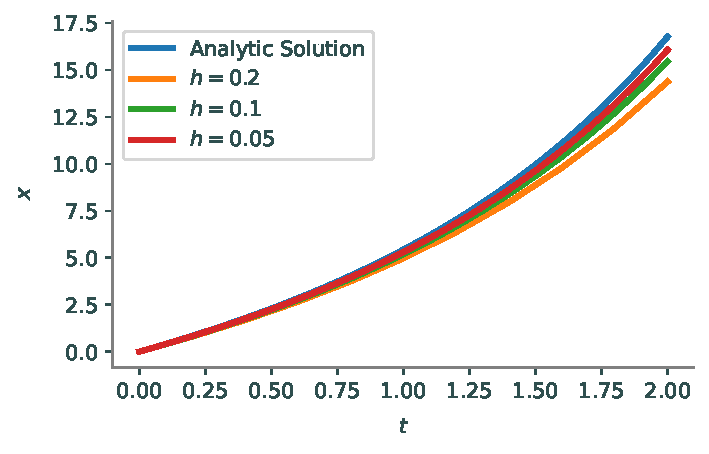
\includegraphics[width=150mm]{figures/euler.pdf}
\caption{The solution of \eqref{ivp:prob1}, alongside several approximations using Euler's method.}
\label{ivp:euler}
\end{figure}

\begin{problem} Write a function which implements Euler's method for an IVP of the form \eqref{ivp:generic}. Test your function on the IVP:
\begin{align}
	\begin{split}
		x' (t)&= x(t) - 2t + 4,\quad 0 \leq t \leq 2, \\
		x(0) &= 0,
	\end{split}\label{ivp:prob1}
\end{align}
where the analytic solution is $x(t) = -2+2t + 2e^t.$
Use the Euler method to numerically approximate the solution with step sizes $h = 0.2, 0.1$, and $0.05.$ Plot the true solution alongside the three approximations, and compare your results with Figure \ref{ivp:euler}.
\end{problem}



\subsection*{Midpoint Method}

The midpoint method is very similar to Euler's method.
For small $h$, use the approximation
\begin{align*}
\x(t_{i+1}) &\approx  \x(t_{i}) + h f(\x(t_{i})+\frac{h}{2} f(\x(t_i),t_i),t_{i}+\frac{h}{2}).
\end{align*}
In this approximation, first set $\hat \x_i = \x_i+\frac{h}{2}f(\x_i,t_i)$, which is an Euler method step of size $h/2$.
Then evaluate $f(\hat \x_i,t_i+\frac{h}{2})$, which is a more accurate approximation to the derivative $\x'(t)$ in the interval $[t_i,t_{i+1}]$.
Finally, a step is taken in that direction, scaled by $h$.
It can be shown that the local truncation error for the midpoint method is $\mathcal{O}(h^3)$, giving global truncation error of $\mathcal{O}(h^2)$.
This is a significant improvement over the Euler method.
However, it comes at the cost of additional evaluations of $f$ and a handful of extra floating point operations on the side.
This tradeoff will be considered later in the lab.

\subsection*{Runge-Kutta Methods}
The Euler method and the midpoint method belong to a family called \textit{Runge-Kutta methods}.
There are many Runge-Kutta methods with varying orders of accuracy.
Methods of order four or higher are most commonly used.
A fourth-order Runge-Kutta method (RK4) iterates as follows: 
\begin{align*}
	\begin{split}
K_1 &= f(\x_i,t_i), \\
K_2 &= f(\x_i + \frac{h}{2} K_1,t_i + \frac{h}{2}),\\
K_3 &= f(\x_i + \frac{h}{2} K_2,t_i + \frac{h}{2}),\\
K_4 &= f(\x_i + h K_3,t_{i+1}),\\
\x_{i+1} &= \x_i + \frac{h}{6}(K_1 + 2K_2 + 2K_3 + K_4).
	\end{split}
\end{align*}

Runge-Kutta methods can be understood as a generalization of quadrature methods for approximating integrals, where the integrand is evaluated at specific points, and then the resulting values are combined in a weighted sum.
For example, consider a differential equation 
$$x'(t) = f(t)$$
Since the function $f$ has no $x$ dependence, this is a simple integration problem.
In this case, Euler's method corresponds to the left-hand rule, the midpoint method becomes the midpoint rule, and RK4 reduces to Simpson's rule.

\section*{Advantages of Higher-Order Methods}
It can be useful to visualize the order of accuracy of a numerical method.
A method of order p has relative error of the form
$$E(h) = Ch^p$$
taking the logarithm of both sides yields
$$log(E(h)) =p \cdot log(h) + log(C)$$
Therefore, on a log-log plot against $h$, $E(h)$ is a line with slope $p$ and intercept $log(C)$.

\begin{problem} Write functions that implement the midpoint and fourth-order Runge-Kutta methods.
Use the Euler, Midpoint, and RK4 methods to approximate the value of the solution for the IVP \eqref{ivp:prob1} from Problem 1 for step sizes of $h = 0.2,$ $ 0.1,$ $0.05 $, $0.025,$ and $0.0125.$

Plot the following graphs
\begin{itemize}
\item The true solution alongside the approximation obtained from each method when $h=0.2$.
\item A log-log plot (use \li{plt.loglog}) of the relative error $|x(2)-x_n|/{|x(2)|}$ as a function of $h$ for each approximation.
\end{itemize}

Compare your second plot with Figure \ref{ivp:relative_error}.
\end{problem}

\begin{figure}[H]
\centering
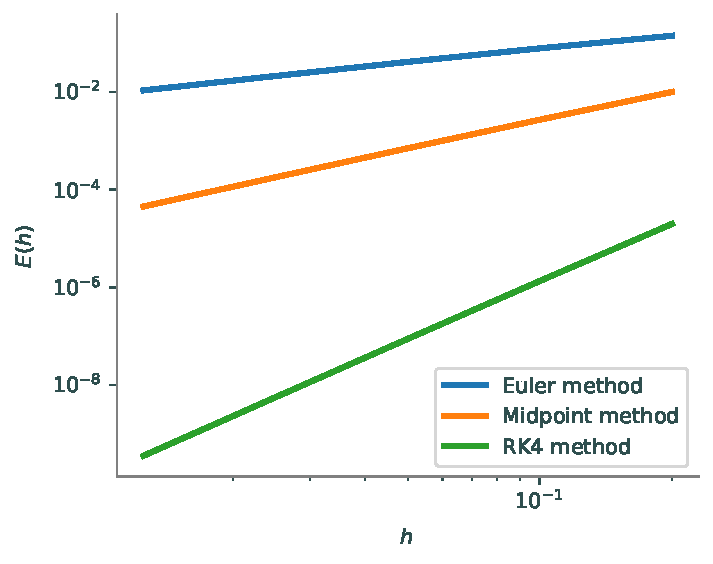
\includegraphics[width=\textwidth]{figures/prob2.pdf}
\caption{Loglog plot of the relative error in approximating $x(2)$, using step sizes $h = 0.2,$ $0.1,$ $0.05,$ $0.025,$ and $0.0125$.
The slope of each line demonstrates the first, second, and fourth order convergence of the Euler, Midpoint, and RK4 methods, respectively.}
\label{ivp:relative_error}
\end{figure}

The Euler, midpoint, and RK4 methods help illustrate the potential trade-off between order of accuracy and computational expense.
To increase the order of accuracy, more evaluations of $f$ must be performed at each step.
It is possible that this trade-off could make higher-order methods undesirable, as (in theory) one could use a lower-order method with a smaller step size $h$.
However, this is not generally the case.
Assuming efficiency is measured in terms of the number of $f$-evaluations required to reach a certain threshold of accuracy, higher-order methods turn out to be much more efficient.
For example, consider the IVP

\begin{align}
	\begin{split}
		x'(t) &= x(t) \cos(t), \quad t \in [0,8],\\
		x(0) &= 1. 
	\end{split}
	\label{ivp:efficiency_problem}
\end{align}
Figure \ref{ivp:efficiency_figure} illustrates the comparative efficiency of the Euler, Midpoint, and RK4 methods applied to \eqref{ivp:efficiency_problem}. 
The higher-order RK4 method requires fewer $f$-evaluations to reach the same level of relative error as the lower-order methods.
As $h$ becomes small, which corresponds to increasing functional evaluations, each method reaches a point where the relative error $|x(8)-x_n|/{|x(8)|}$ stops improving.
This occurs when $h$ is so small that floating point round-off error overwhelms local truncation error. Notice that the higher-order methods are able to reach a better level of relative error before this phenomena occurs.

\begin{figure}[H]
\centering
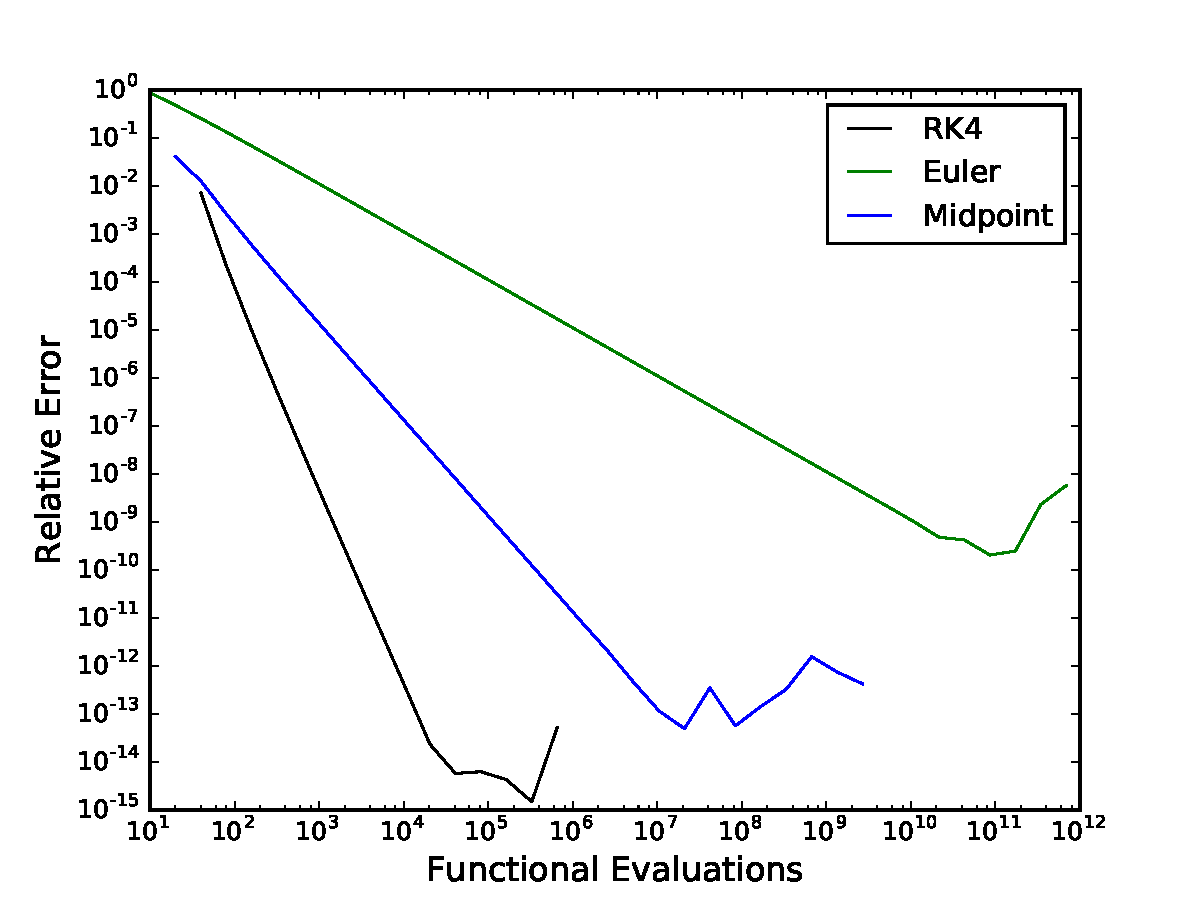
\includegraphics[width=\textwidth]{figures/Efficiency.pdf}
\caption{The relative error in computing the solution of \eqref{ivp:efficiency_problem} at $x = 8$ versus the number of times the right-hand side of \eqref{ivp:efficiency_problem} must be evaluated.  }
\label{ivp:efficiency_figure}
\end{figure}

\begin{comment}
Let $t^*$ be an approximation of some value $t$.
The relative error of the approximation is 
\[ \frac{|t^*-t|}{|t|}.
\]
Note that the relative error is simply the absolute error $|t^*-t|$ normalized by the size of $t$.
A method with order $p$ has error of the form 
\[E(h) = C h^p. \]
This means that the graph of $\log (E)$ versus $\log(h)$ has slope $p$.  
The relative error of a numerical method can be approximated and graphed to verify that $p$th order convergence is occurring. For example, consider the IVP
 \begin{align}
 	\begin{split}
 y' &= y - 2x + 4,\quad 0 \leq x \leq 2, \\
 y(0) &= 0.
 	\end{split} \label{ivp:prob2}
 \end{align}
The following code solves the initial value problem on several grids using the Euler method, approximates the relative error in computing $y(2)$ and creates a plot (see Figure \ref{ivp:relative_error}).

\begin{lstlisting}
import matplotlib.pyplot as plt

a, b, ya = 0., 2., 0.

def ode_f(x,y):
	return np.array([y - 2*x + 4.])
	
best_grid = 320					#  number of subintervals in most refined grid
h = 2./best_grid
X, Y, h, n = initialize_all(a, b, ya, h)
# Requires an implementation of the euler method
best_val = euler(ode_f, X, Y, h, n)[-1]  

smaller_grids = [10, 20, 40, 80]  # number of subintervals in smaller grids
h = [2./N for N in smaller_grids]

Euler_sol = [euler(ode_f, initialize_all(a, b, ya, h[i])[0],
			initialize_all(a, b, ya, h[i])[1], h[i], N+1)[-1]
			for i, N in enumerate(smaller_grids)]
Euler_error = [abs((val - best_val)/best_val) for val in Euler_sol]
	
plt.loglog(h, Euler_error, '-b', label="Euler method", linewidth=2.)
plt.show()

\end{lstlisting}
\end{comment}

\section*{Harmonic Oscillators and Resonance}
Harmonic oscillators are common in classical mechanics.
A few examples include the pendulum (with small displacement), spring-mass systems, and the flow of electric current through various types of circuits.
A harmonic oscillator $y(t)$\footnote{It is customary to write $y$ instead of $y(t)$ when it is unambiguous that $y$ denotes the dependent variable.} is a solution to an initial value problem of the form 
\begin{align*}
	&{}my'' + \gamma y' + ky = f(t) ,\\
	&{}y(0) = y_0,\quad
	y'(0) = y'_0.
\end{align*}
Here, $m$ represents the mass on the end of a spring, $\gamma$ represents the effect of damping on the motion, $k$ is the spring constant, and $f(t)$ is the external force applied.
\begin{comment}
We will describe the construction of this mathematical model in the context of a spring-mass system.

Suppose an object with mass $m$ is placed at the end of a horizontal spring.
The natural position of the object is called the \textit{equilibrium position} for the system.
If the object is displaced from its equilibrium position and given an initial velocity,
it will act like a harmonic oscillator.
The principal property of a harmonic oscillator $y(t)$ is that once $y$ leaves its equilibrium value $y = 0$, it experiences a restoring force $F_r = -ky.$
This force pushes $y$ back towards its equilibrium.
Hooke's law says that this holds true for a
spring-mass system if the displacement $y$ is small.

Often there is an additional damping force $F_d$, often due to some type of friction. 
This force is usually proportional to the $y'$ (the \emph{velocity}), is always in the opposite direction of $y'$, and represents energy leaving the system. (You can think of it as drag.)
Thus we have $F_d = -\gamma y', $ where $ \gamma \geq 0$ is constant.
We may also need to consider an additional external force $f(t)$, or a driving force, that is interacting with our spring-mass system.

By using Newton's law we obtain
\begin{align*}
ma &= F = F_r + F_d + f(t),\\
my'' &= -ky -\gamma y' + f(t).
\end{align*}
\end{comment}

\section*{Simple harmonic oscillators}
A simple harmonic oscillator is a harmonic oscillator that is not damped, $\gamma =0$, and is free, $f = 0$, rather than forced, $f \not = 0$. 
A simple harmonic oscillator can described by the IVP
\begin{align*}
&{}my'' + ky = 0,\\
&{}y(0) = y_0,\quad
y'(0) = y_0'.
\end{align*}
The solution of this IVP is $y = c_1\cos (\omega_0 t) + c_2 \sin (\omega_0 t)$, where $\omega_0 = \sqrt{k/m}$ is the natural frequency of the oscillator and $c_1$ and $c_2$ are determined by applying the initial conditions.

To solve this IVP using a Runge-Kutta method, it must be written in the form
\[\x'(t) = f(\x(t),t) \]
This can be done by setting $x_1 = y \ \text{and} \ x_2 = y'$. Then we have \[     \x'=
 \left[\begin{array}{c}x_1 \\x_2\end{array}\right]'  =  \left[\begin{array}{c}x_2 \\\frac{-k}{m}x_1\end{array}\right]\]
Therefore$$f(\x(t),t) = \left[\begin{array}{c}x_2 \\\frac{-k}{m}x_1\end{array}\right]$$

\begin{problem} Use the RK4 method to solve the simple harmonic oscillator satisfying 
\begin{align}
	\begin{split}
&{}my'' + ky = 0,\quad 0 \leq t \leq 20, \\
&{}y(0) = 2, \quad
y'(0) = -1,
	\end{split}
	\label{ivp:simple_oscillator}
\end{align}
for $m = 1$ and $k =1$.

Plot your numerical approximation of $y(t)$.  
Compare this with the numerical approximation when $m = 3$ and $k =1$. Consider: Why does the difference in solutions make sense physically?
\end{problem}


\begin{figure}[H]
\centering
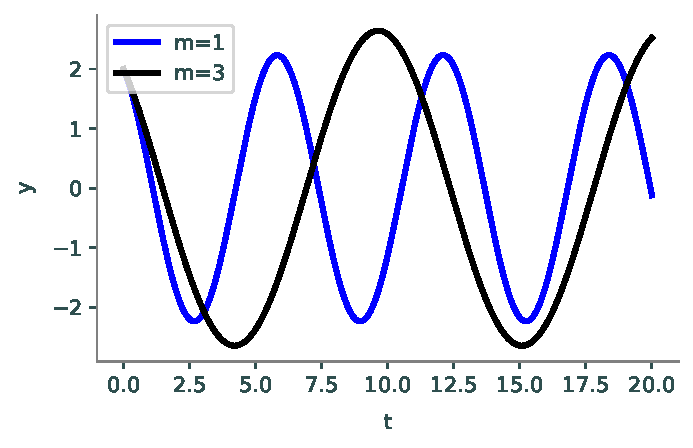
\includegraphics[width=\textwidth]{figures/simple_oscillator.pdf}
\caption{Solutions of \eqref{ivp:simple_oscillator} for several values of $m$.}
\label{ivp:simple_oscillator_figure}
\end{figure}


\section*{Damped free harmonic oscillators} 
A damped free harmonic oscillator $y(t)$ satisfies the IVP
\begin{align*}
	&{}my'' + \gamma y' + ky = 0 ,\\
	&{}y(0) = y_0,\quad
	y'(0) = y'_0.
\end{align*}
\begin{comment}
For fixed values of $m$ and $k$, it is interesting to study the effect of the damping coefficient $\gamma$.
\end{comment}

The roots of the characteristic equation are \[r_1,r_2 = \frac{-\gamma \pm \sqrt{\gamma^2 -4km}}{2m} .\]
Note that the real parts of $r_1$ and $r_2$ are always negative, and so any solution $y(t)$ will decay over time due to a dissipation of the system energy. 
There are several cases to consider for the general solution of this equation:
\begin{enumerate}
\item If $\gamma^2 > 4km$, then the general solution is $y(t) = c_1 e^{r_1t} + c_2e^{r_2t}$. Here the system is said to be $\textit{overdamped}$. 
Notice from the general solution that there is no oscillation in this case.
\item If $\gamma^2 = 4km$, then the general solution is $y(t) = c_1 e^{\gamma t/2m} + c_2 te^{\gamma t/2m}$. Here the system is said to be $\textit{critically damped}$.
\item If $\gamma^2 < 4km$, then the general solution is
\begin{align*}
y(t) &= e^{-\gamma t/2m} \left[c_1\cos(\mu t) + c_2 \sin (\mu t)\right],\\
&= R e^{-\gamma t/2m}  \sin (\mu t + \delta),
\end{align*}
where $R$ and $\delta$ are fixed, and $\mu = \sqrt{4km-\gamma^2}/2m.$ This system does oscillate.
\end{enumerate}

\begin{problem}
Use the RK4 method to solve for the damped free harmonic oscillator satisfying 
\begin{align*}
&{}y'' +\gamma y'+ y = 0, \quad 0 \leq t \leq 20,\\
&{}y(0) = 1, \quad
y'(0) = -1.
\end{align*}
For $\gamma = 1/2,$ and $\gamma = 1$, simultaneously plot your numerical approximations of $y$.
\end{problem}

\section*{Forced harmonic oscillators without damping}
Consider the systems described by the differential equation
\begin{align}
my''(t)  + ky(t) &= F(t). \label{Forced_harm_osc}
\end{align}
In many instances, the external force $F(t)$ is periodic, so assume that $F(t) = F_0 \cos(\omega t)$. 
If $\omega_0 = \sqrt{k/m} \not = \omega,$ then the  general solution of \ref{Forced_harm_osc} is given by
\[y(t) = c_1 \cos (\omega_0 t) + c_2\sin (\omega_0 t) + \frac{F_0}{m(\omega_0^2 - \omega^2)} \cos (\omega t).\]
If $\omega_0 = \omega$, then the general solution is
\[y(t) = c_1 \cos (\omega_0 t) + c_2\sin (\omega_0 t) + \frac{F_0}{2m\omega_0} t \sin (\omega_0 t).\]

When $\omega_0 = \omega$, the solution contains a term that grows arbitrarily large as $t \to \infty$.
If we included damping, then the solution would be bounded but large for small $\gamma$ and $\omega$ close to $\omega_0$.

Consider a physical spring-mass system.
Equation \ref{Forced_harm_osc} holds only for small oscillations; this is where Hooke's law is applicable.
However, the fact that the equation predicts large oscillations suggests the spring-mass system could fall apart as a result of the external force. 
This mechanical resonance has been known to cause failure of bridges, buildings, and airplanes.

\begin{problem}
Use the RK4 method to solve the damped and forced harmonic oscillator satisfying 
\begin{align}
	\begin{split}
&{}2y'' + \gamma y' + 2y = 2 \cos (\omega t), \quad 0 \leq t \leq 40,\\
&{}y(0) = 2, \quad
y'(0) = -1. 
	\end{split}
	\label{ivp:damped_forced_oscillator}
\end{align}
For the following values of $\gamma$ and $\omega,$ plot your numerical approximations of $y(t)$: $(\gamma, \omega) = (0.5, 1.5),$ $(0.1, 1.1),$ and $(0, 1)$.
Compare your results with Figure\ref{ivp:damped_forced_oscillator}.
\end{problem}


\begin{figure}[H]
\centering
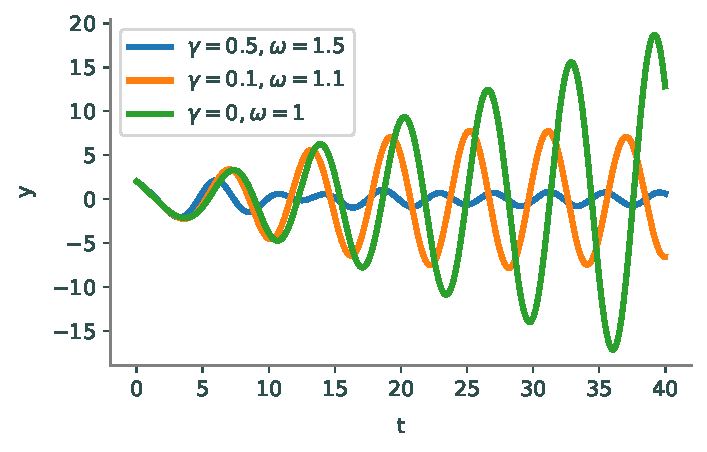
\includegraphics[width=\textwidth]{figures/damped_forced_oscillator.pdf}
\caption{Solutions of \eqref{ivp:damped_forced_oscillator} for several values of $\omega$ and $\gamma$.}
\label{ivp:damped_forced_oscillator_figure}
\end{figure}
